\documentclass[a4paper, 10pt]{report}

\usepackage{graphicx}

\usepackage{hyperref}


\usepackage{geometry}
 \geometry{
 a4paper,
 total={170mm,257mm},
 left=22mm,
 top=22mm,
 }


\title{Report}
\author{Subham Kumar}
\date{}
\begin{document}
\maketitle

\listoffigures


 





\begin{figure}
\centering
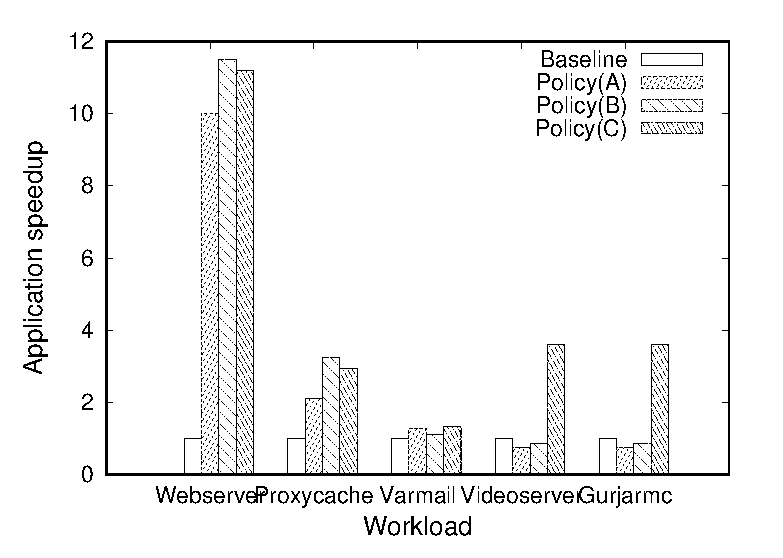
\includegraphics[width=\columnwidth]{speedup.eps}

 \label{fig:figr1}
\end{figure}





\begin{figure}
\centering

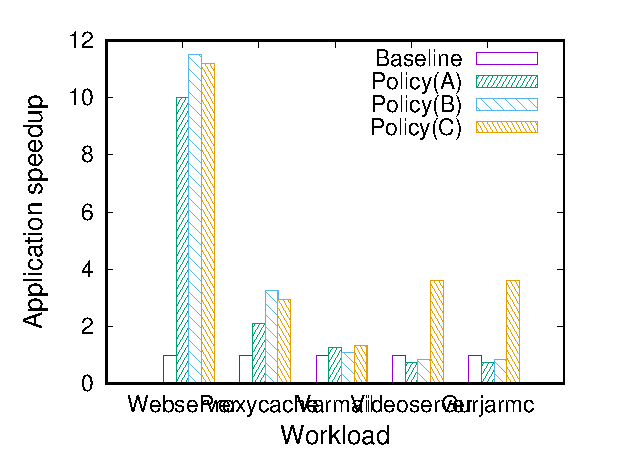
\includegraphics[width=\columnwidth]{speedup_color.eps}
 \label{fig:figr2}
\end{figure}


\begin{figure}
\centering

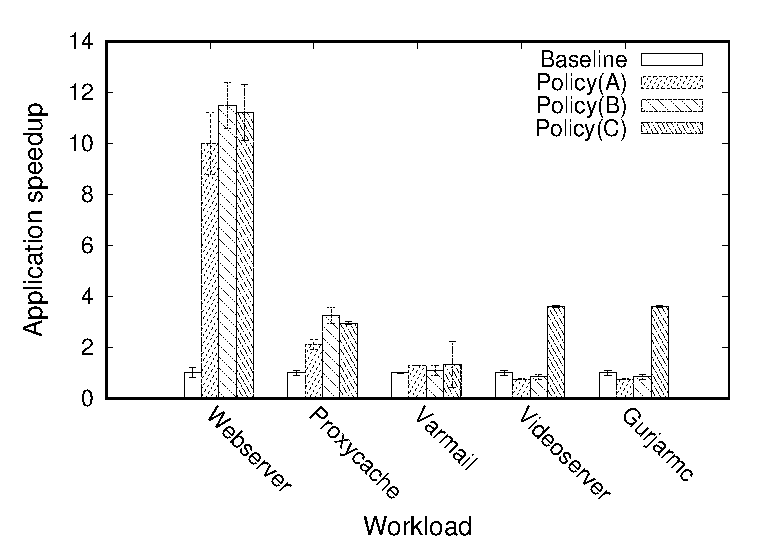
\includegraphics[width=\columnwidth]{speedup_errorbar.eps}
 \label{fig:figr3}
\end{figure}

\begin{figure}
\centering
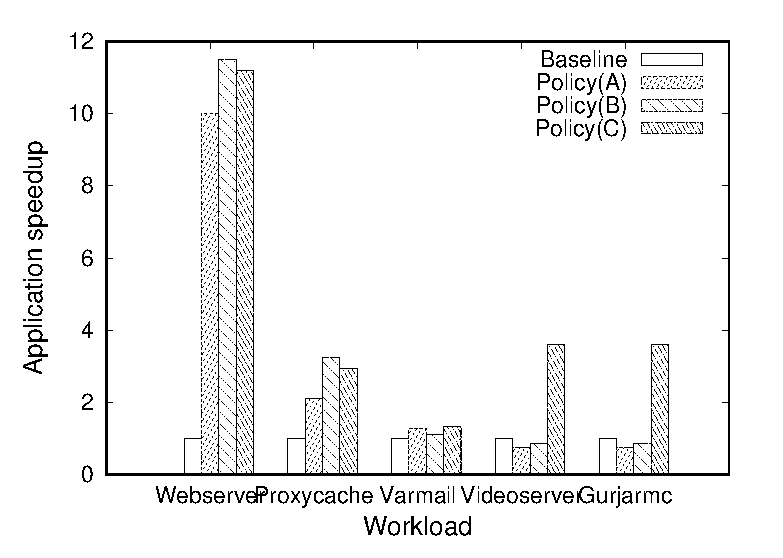
\includegraphics[width=\columnwidth]{speedup.eps}
 \label{fig:figr4}
\end{figure}


\begin{figure}
\centering
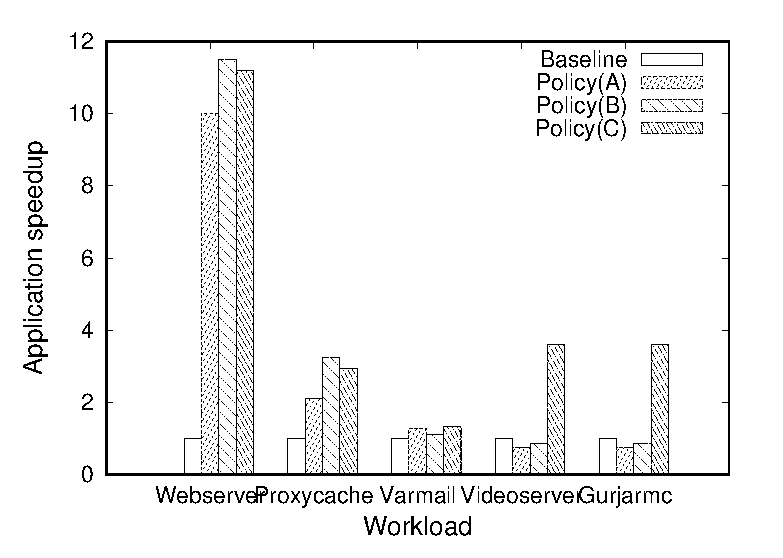
\includegraphics[width=\columnwidth]{speedup.eps}
 \label{fig:figr5}
\end{figure}


\begin{figure}
\centering
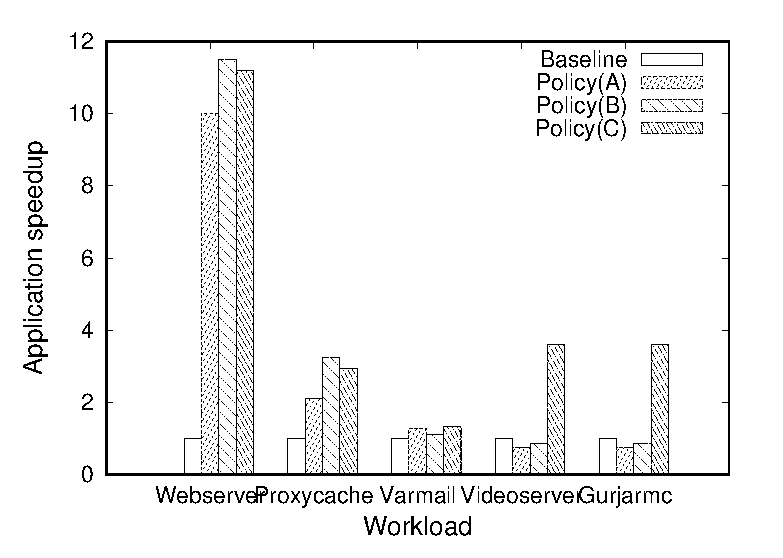
\includegraphics[width=\columnwidth]{speedup.eps}
 \label{fig:figr6}
\end{figure}


\begin{figure}
\centering
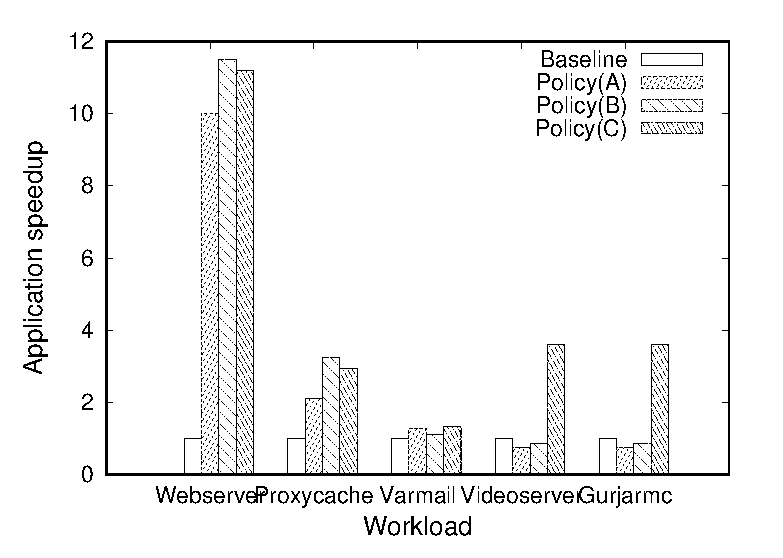
\includegraphics[width=\columnwidth]{speedup.eps}
 \caption{speedup}
 \label{fig:figr7}
\end{figure}



\begin{figure}
\centering
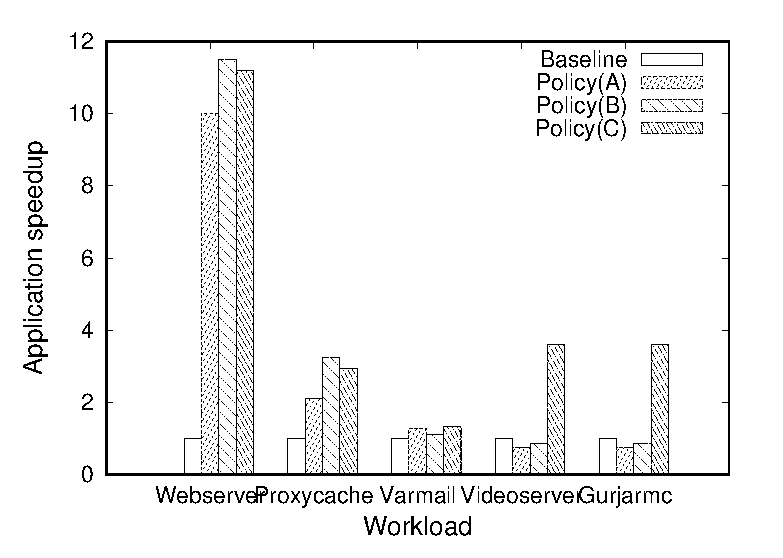
\includegraphics[width=\columnwidth]{speedup.eps}
 \caption{speedup}
 \label{fig:figr8}
\end{figure}



\begin{figure}
\centering
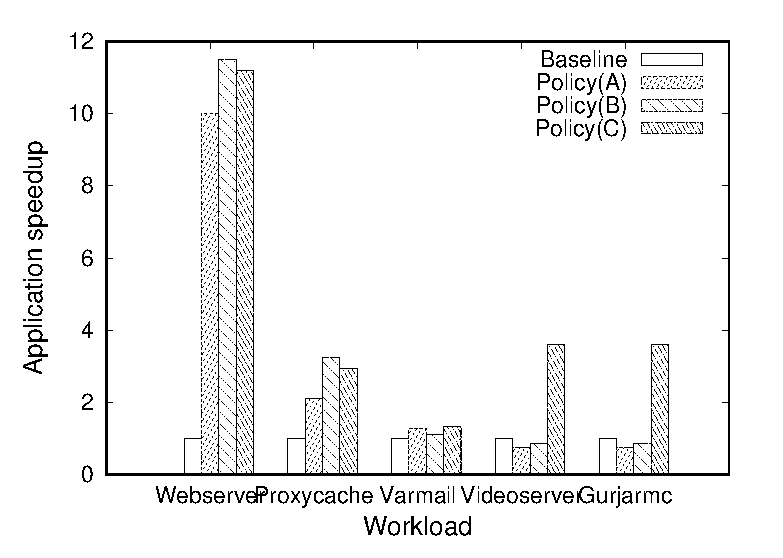
\includegraphics[width=\columnwidth]{speedup.eps}
 \caption{speedup}
 \label{fig:figr9}
\end{figure}






\end{document}
